\documentclass[12pt,twoside]{book}
\usepackage[utf8]{inputenc}
\usepackage[T1]{fontenc}
\usepackage{natbib}
\usepackage[francais]{babel}
\usepackage[toc,page]{appendix} 
\usepackage{graphicx}
\usepackage{geometry}
\usepackage{xcolor}
\usepackage{listings}
\usepackage{natbib}
\pagestyle{plain}
\geometry{top=2.5cm, bottom=3.5cm, left=3cm , right=2cm}
\renewcommand{\thechapter}{\Roman{chapter}}
\renewcommand{\thesection}{\Alph{section}}

\newcommand{\LMUTitle}[9]{
  \thispagestyle{empty}
  \vspace*{\stretch{1}}
  {\parindent0cm
   \rule{\linewidth}{.7ex}}
  \begin{flushright}

    \vspace*{\stretch{1}}
    \sffamily\bfseries\Huge
    #1\\
    \vspace*{\stretch{1}}
    \sffamily\bfseries\large
    #2
    \vspace*{\stretch{1}}
  \end{flushright}
  \rule{\linewidth}{.7ex}
  \vspace*{\stretch{5}}
  \begin{center}
    
\includegraphics[width=3in]{UPN-logo.jpg}
  \end{center}
  \vspace*{\stretch{1}}
  \begin{center}\sffamily\LARGE{#3}\end{center}
  \newpage
  \thispagestyle{empty}
}

\begin{document}

  \LMUTitle
      {Génération automatique\\
      de tests}              
      {Lucas Nayet}                       
      {Juin 2018}                          

\thispagestyle{empty}
\setcounter{page}{0}
J'adresse mes remerciements à mon responsable de stage, Monsieur François Delbot, pour l'aide et le temps qu'il m'a consacré ainsi qu'à mon tuteur enseignant, Monsieur Souheib Baarir.\\
Je tiens également à remercier Monsieur Pascal Poizat, responsable de la MIAGE M1 classique.\\
J'adresse également mes remerciements à la formation MIAGE de l'UFR SEGMI qui m'a accueilli cette année pour ma première année de master et à toute l'équipe éducative.\\
Enfin, je tiens à remercier toutes les personnes qui m'ont aidé d'une manière ou d'une autre à la réalisation de ce stage.

\tableofcontents

\color{red}
\chapter{Présentation du stage}
\color{black}
\section {Les circonstances du stage}
Étant étudiant à l'UFR Segmi de l'Université Paris Nanterre en M1 MIAGE, je devais effectuer un stage nécessaire pour la validation de mon M1 et mon passage en Master 2 MIAGE.\\ 
N'ayant malheureusement pas trouvé d'entreprise, le stage s'est donc déroulé dans mon université, à Nanterre. Mon responsable de stage fut donc un de mes enseignants, Monsieur François Delbot, qui m'a donné les différentes directives à suivre durant toute la durée du stage.

\section {En quoi consiste le stage ?}
\subsection{Contexte}
Les L1 et L2 ont un taux d'échec très important en programmation. Cela est lié à plusieurs facteurs : l'absentéisme, le manque de suivi qui est très présent à l'université et le gros contraste de niveau en fonction des filières que les étudiants ont effectuées au lycée.\\
Pour lutter contre ce taux d'échec, Monsieur Jean-François Pradat Peyre et Monsieur François Delbot, enseignants chercheurs à l'université Paris X ont imaginé et développé la plate-forme Cat qui va permettre aux étudiants de s'auto-évaluer (évaluation formative) et d'être évalués (évaluation sommative).\\
En effet, Cat permet de créer un cours, un td, un exercice... et
permet de corriger automatiquement les exercices via des tests utilisant des variables booléennes : retourne 1 quand le test passe et 0 quand le test ne passe pas.\\
Cat représente donc un gain de temps très important pour les enseignants car les corrections se font automatiquement.\\
Ainsi, Cat facilite l'évaluation des étudiants et permet à ces derniers de progresser à leur rythme, cela n'étant pas chose aisée en cours où il faut suivre le rythme du professeur.\\
Cependant, actuellement, la plateforme ne gère que les exercices qui sont codés en langage C. Le but du stage est donc de pouvoir permettre à Cat d'accepter un second langage, le HTML.\\
\subsection{Synopsis du stage}
Le stage porte donc sur la génération de tests pour des fichiers HTML dans le langage de programmation Python.\\On part d'un fichier de référence que l'on appellera ici "modele.html" et à partir de ce dernier, nous allons générer une série de tests qui permettront à d'autres fichiers html d'être comparés avec le fichier de référence pour savoir s'ils sont valides ou non.

\section {Les pré-requis}
Pour effectuer cela, quelques préparatifs étaient indispensables.
\subsection{L'environnement de travail}
Le système d'exploitation sur lequel je devais travailler était Linux. On l'obtient via la virtualisation avec un logiciel comme VirtualBox par exemple ou encore en mettant son ordinateur en DualBoot. Pour le stage, la virtualisation a été privilégiée.\\
Ensuite, pour pouvoir faire le fond du stage (sur lequel on va s'attarder dans le chapitre suivant), je devais utiliser la bibliothèque Beautiful Soup.
\subsection{Installer Beautiful Soup}
Pour installer Beautiful Soup, rendez-vous dans un terminal et saisissez avant toute installation quelconque la commande suviante : \textbf{sudo apt-get update} qui permettra de mettre à jour votre système. Ensuite, vous pourrez saisir ce qui vous permettra d'installer la bibliothèque voulue soit \textbf{sudo pip install beautifulsoup4} si pip n'est pas reconnu, c'est qu'il n'est pas installé. Pour l'installer, faites la commande suivante : \textbf{sudo apt-get install python-pip} et une fois installé, refaites la commande précédente. Beautiful Soup est donc installée et prête à être utlisée.

\color{red}
\chapter{Les enjeux du stage}
\color{black}
\section{Le fichier HTML de référence}
\lstinputlisting{modele.html}
Ce fichier sera le fichier de référence pour générer les tests.\\ Les fichiers étudiants devront comporter les mêmes éléments, les mêmes balises et les paragraphes par exemple devront avoir le même contenu.\\ 
Cependant, les fichiers pourront avoir du contenu supplémentaire par rapport à celui de référence. L'important est que le contenu présent dans le fichier modèle soit présent dans les fichiers étudiants. \\
Les tests serviront donc à vérifier cela. 
\newpage
\section{Le parsing de HTML}
Pour pouvoir faire le script Python permettant de générer les tests automatiquement, il va falloir parser de l'HTML. Parser signifie analyser, le but ici est donc d'analyser les balises HTML et leur contenu (du fichier modèle) et pouvoir comparer cela aux fichiers étudiants.\\
Et c'est là que la bibliothèque Beautiful Soup entre en jeu ! Elle permet, en effet, de parser de l'HTML.\\
Pour pouvoir utiliser Beautiful Soup dans notre script Python, il faut mettre en début de programme la ligne suivante : \textbf{from bs4 import BeautifulSoup}.\\
Ensuite, on doit associer un document html au parseur et cela se fait avec la ligne de code suivante : \textbf{soup=BeautifulSoup(html\_doc)}\\
Ici, html\_doc est la chaine de caractères qui contiendra le fichier html.\\ \\
La bibliothèque Beautiful Soup permet de récupérer le contenu d'une balise spécifiée, comme par exemple la balise p, celle des paragraphes !\\ Exemple : \textbf{for p in soup.find\_all('p'):} permet de récupérer le contenu de toutes les balises 'p'. On est libre de stocker cela dans une liste par exemple : à chaque tour de boucle, si on fait \textbf{liste.append(p)} alors le contenu de la balise p trouvée viendra s'ajouter à la liste.\\
La bibliothèque Beautiful Soup permet d'autres choses comme par exemple changer le contenu ou remplacer des balises, mais cela ne nous intéresse pas dans le cadre du stage. 

\section{L'approche effectuée}
Le finalité étant d'avoir une série de tests qui s'effectue lorsque l'on rentre un fichier étudiant en paramètre, j'ai décidé d'avoir une approche par palier.\\ En effet, à partir du fichier modèle qui se trouve plus haut, on peut facilement mettre en place une architecture progressive permettant de faire les tests les uns après les autres tout en les rendant dépendants entre eux. Par exemple, le premier test qui semble évident à effectuer est la présence ou non de balise html dans le fichier. Si le test passe, ce qui signifie que le fichier étudiant respecte l'architecture ou le contenu du fichier modèle, alors le test suivant peut être effectué. Dans le cas contraire, cela signifie que le document ne possède pas de balise html et il est inutile de poursuivre les tests dessus: tous les autres tests échoueront puisqu'un document html doit commencer par une balise html et se fermer par cette même balise.\\
Ainsi, en prenant le fichier modèle comme exemple, le premier test à effectuer est donc la présence ou non de la balise html, ensuite la présence ou non de la balise head, ensuite la présence ou non de la balise title, ensuite la vérification du contenu de la balise title entre le fichier modèle et celui étudiant et ainsi de suite...\\
Une nouvelle fois, si par exemple le test de la présence de la balise title est rejeté, alors il est inutile de vérifier le contenu de cette dernière, elle n'existe simplement pas. Il faut effectuer des tests seulement là où c'est utile de le faire.

\color{red}
\chapter{ La réalisation du stage}
\color{black}
\section{Le script des tests}
Le script Python dans lequel l'on va coder l'ensemble des tests s'appelle "test.py". Ce fichier, disponible avec les sources, est le fichier où tout les tests sont codés.\\
Cependant, la première fonction est une fonction permettant de récupérer le fichier HTML que l'on rentre en paramètre via une chaîne de caractère; en effet, cela est nécessaire pour pouvoir permettre à Beautiful Soup de pouvoir faire son travail de parsing dessus et donc d'appliquer les tests dessus. \\
Sinon toutes les autres fonctions présentes sont des fonctions qui permettent de réaliser des tests booléens. Ici, deux catégories de tests se dégagent : ceux qui permettent de savoir si une balise est présente ou non et l'autre qui permet de savoir si le contenu de la balise est fidèle au contenu de la balise du fichier de référence.\\
La fonction "verifier\_presence\_balise\_paragraphe()" par exemple, appartient à la première catégorie. En voici le code : \\
\begin{lstlisting}
def verifier_presence_balise_paragraphe():
	cpt_etudiant=0
	cpt_modele=0
	for paragraphe in soupmodele.html.body.find_all('p'):
		cpt_modele+=1
	for paragraphe in soupetudiant.html.body.find_all('p'):
		cpt_etudiant+=1
	if cpt_etudiant>=cpt_modele and cpt_etudiant!=0: return 1
	return 0
\end{lstlisting}
Quelques explications : \\
Le "soupmodele.html.body.find\_all('p')" permet de rechercher la présence de balise p dans le fichier modèle (et pour le fichier étudiant avec soupetudiant), le find\_all permet d'indiquer que toutes les balises (et pas seulement une) vont être recherchées. Par ailleurs, les balises vont être recherchées dans la balise body qui elle-même est dans la balise html, cela respecte l'approche par palier évoquée plus haut, ce test ne sera effectué que si la balise body a été trouvée, en effet, on ne peut pas trouver de balise dans une balise qui n'existe pas. Ensuite, on compte le nombre de balises p trouvées via les compteurs modèle et étudiant et on les compare ensuite via un if. Si le compteur étudiant est supérieur ou égal à celui du compteur modèle, alors le nombre de paragraphes est respecté. Il faut néanmoins vérifier qu'il ne vaut pas 0 car cela voudrait dire qu'il n'y a pas de balise p. Ainsi, on peut retourner 1 si c'est le cas et valider par conséquent le test.\\
Maintenant, si la présence et le nombre de paragraphes a été validé, il va falloir effectuer la vérification du contenu des paragraphes et cela appartient à la seconde catégorie de tests dont voici le code ci-dessus : \\
\begin{lstlisting}
def verifier_contenu_balise_paragraphe():
	liste_modele=[]
	liste_etudiant=[]
	i=0
	j=0
	k=0
	t=0
	validator=0
	for b in soupmodele.html.body.find_all('p'):
		liste_modele.append(b.string)
		j+=1
	for b in soupetudiant.html.body.find_all('p'):
		liste_etudiant.append(b.string)	
		t+=1	
	while i<j: 
		if liste_modele[i]!=liste_etudiant[i]:		
			break
		i+=1
	if i==j: return 1 
	else: 	
		while(k<t):
			i=0
			while(i<j): 
				if liste_etudiant[k]==liste_modele[i]: 
					validator+=1
					break
				i+=1
			k+=1
		if validator==j: return 1
		return 0
\end{lstlisting}
La première partie du code est assez simple, on récupère le contenu des paragraphes dans des listes puis on les compare entre elles et on s'arrête si on trouve une différence car cela signifie que les étudiants n'ont pas respecté le modèle. Dans le cas contraire, on retourne 1 et le test passe. Cependant, et c'est là la subtilité, on tolère le fait que les paragraphes soient présents dans un ordre différent de celui du fichier modèle et c'est pour cela que l'on fait une double boucle while qui permet de vérifier si les paragraphes sont présents dans un ordre différent chez l'étudiant ou non. Si c'est le cas, on retourne 1 et le test est validé, dans le cas contraire on retourne 0 et le test est rejeté.\\
La tolérance est également valable pour les balises div et img.\\ \\
A noter que l'on trouve en fin de fichier les instructions permettant de récupérer les fichiers HTML et de pouvoir les parser avec Beautiful Soup, les voici ci-dessous :\\
\begin{lstlisting}
etudiant="etudiant.html"
modele="modele.html"
html_modele = charger_fichier_html(modele)
html_etudiant = charger_fichier_html(etudiant)
soupmodele = BeautifulSoup(html_modele,"lxml")
soupetudiant = BeautifulSoup(html_etudiant,"lxml")
\end{lstlisting}

\section{Le script générant les tests}
La génération des tests n'a pas lieu dans le même fichier Python que celui où les tests sont codés. Elle a en effet lieu dans un fichier séparé, appelé "application.py" pour les besoins du stage. \\
Ce fichier prendra les tests du fichier "test.py" pour les générer. Ce dernier sera donc une bibliothèque pour le fichier "application.py", on appelle aussi cela un module. Pour ce faire, il suffit de mettre au début du code dans le fichier "application.py" la ligne suivante : \textbf{from test import *} qui permettra au fichier "application.py" d'avoir accès aux fonctions et variables du fichier "test.py" et de pouvoir les réutiliser sans les recoder.\\
Le code de ce script est disponible avec les sources. On génère les tests en appelant les différentes fonctions qui sont codées sur le fichier "test.py". Pour les besoins du stage, deux fichiers html sont soumis aux tests : "etudiant.html" et "etudiant2.html". Ci-dessous, les codes de ces fichiers :
\newpage
etudiant.html:
\lstinputlisting{etudiant.html}
etudiant2.html:
\lstinputlisting{etudiant2.html}
\newpage
Les tests générés donnent respectivement pour les deux fichiers :
\begin{figure}[h]
\begin{center}
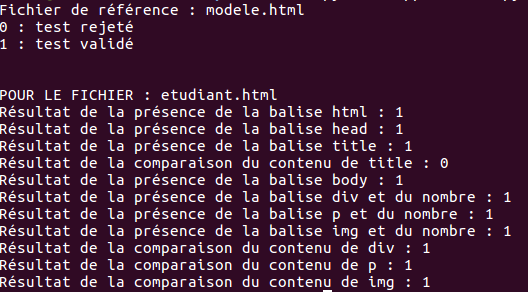
\includegraphics[width=120mm]{generationetudiant1.png}
\caption{Génération pour l'étudiant 1}
\label{fig:génération pour l'étudiant 1}
\end{center}
\end{figure}
\\Ici, tous les tests passent à l'exception de la comparaison du titre, ce qui est cohérent : le titre de l'étudiant 1 n'est pas le même que celui du modèle.
\begin{figure}[h]
\begin{center}
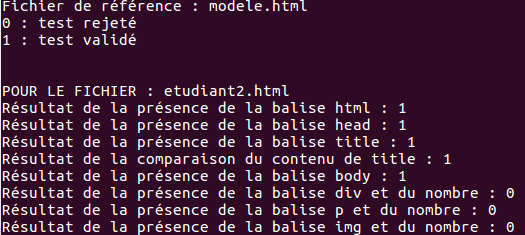
\includegraphics[width=120mm]{generationetudiant2.png}
\caption{Génération pour l'étudiant 2}
\label{fig:génération pour l'étudiant 2}
\end{center}
\end{figure}
\\Ici, c'est différent. Les balises div, p et img sont rejetées. On note en conséquence que les tests de vérification du contenu de ces balises ne sont pas faits, c'est en effet inutile, vu que les balises ont été rejetées. 
\section{Perspectives d'avenir}
Des améliorations sont bien évidemment possibles. L'une d'entre elles est de faire appel à la distance de Levenshtein, qui permettra notamment de rendre les tests non sensibles aux espaces ce qui signifie que le contenu des paragraphes pourra être validé en cas d'espace en trop par rapport à celui du fichier modèle, où encore d'accepter les chemins absolus pour les images s'ils correspondent aux chemins relatifs.\\
On peut aussi regrouper les tests dans un tableau html où le résultat de chaque test (0 ou 1) sera inscrit afin d'avoir une vue plus générale et de pouvoir comparer chaque fichier étudiant pour déterminer plus facilement qui est le meilleur et quel fichier se rapproche le plus du fichier modèle. On peut aussi, en suivant cette logique, de faire une comparaison de tests réussis entre chaque fichier et de qualifier de meilleur le fichier qui a passé le plus de tests.\\ \\
Ces améliorations sont prévues pour la suite mais n'ont pas pu être faites ici, par faute de temps.

\color{red}
\chapter{ Les difficultés rencontrées}
\color{black}
La principale difficulté rencontrée durant ce stage fut le temps. Ayant commencé le stage début Juin à l'université, à la suite de l'échec de mes recherches d'entreprises, je n'avais qu'un mois devant moi pour faire un stage cohérent et rédiger un rapport qui tient la route. Le défi était donc de taille. Je devais en effet, saisir rapidement les enjeux et pouvoir en même temps, faire coïncider rapidité et efficacité.\\ \\
Le fait que les tests ont dû être codés en Python a représenté une difficulté, bien que moindre étant donné que ce langage est plus simple (pour ma part) que les autres. Cependant, certains éléments de la syntaxe, comme les deux points après un if, else, while, for ou encore l'absence de parenthèses dans une condition m'ont conduit à des erreurs dans le programme lorsque je passais dans le terminal. Cela n'a cependant pas été un obstacle gênant dans la réussite du stage, juste une question d'adaptation.

\color{red}
\chapter{Conclusion}
\color{black}
Ce stage m'a été confié dans le but d'améliorer la plate-forme d'évaluation Cat, afin qu'il puisse supporter les fichiers HTML en plus des fichiers C.\\ \\
Le but ici était donc de pouvoir générer des tests à partir de fichiers HTML, un de référence et un étudiant que l'on rentre en paramètres dans un script Python, et de les comparer entre eux afin de valider ou non celui étudiant.\\ \\
Le temps, de seulement un mois aura été un grand défi, et j'ai fait de mon mieux afin de pouvoir le relever.\\ \\
J'espère par la suite, pouvoir aller plus loin que la production que j'ai pu effectuer en un mois.

\chapter*{Webographie}
\begin{description}
\item{[1]} http://www.python-simple.com/python-autres-modules-non-standards/beautifulSoup.php
\item{[2]} http://apprendre-python.com/page-beautifulsoup-html-parser-python-library-xml
\item{[3]} http://sametmax.com/parser-du-html-avec-beautifulsoup/
\item{[4]} https://code.tutsplus.com/fr/tutorials/scraping-webpages-in-python-with-beautiful-soup-the-basics--cms-28211
\item{[5]} https://www.crummy.com/software/BeautifulSoup/bs4/doc/
\item{[6]} https://stackoverflow.com/questions/41720896/python-beautifulsoup-parsing-html


\end{description}

\end{document}
